% Rapport du projet Big Data (4 pages max) -- à compiler sur Overleaf avec pdfLaTeX
% Fichiers à importer dans le projet Overleaf : rapport.tex + schema_pipeline.pdf
\documentclass[10pt,a4paper]{article}

\usepackage{iftex}
\ifPDFTeX            % Overleaf par défaut (pdfLaTeX)
  \usepackage[utf8]{inputenc}
  \usepackage[T1]{fontenc}
  \usepackage{lmodern}
\else                % XeLaTeX / LuaLaTeX
  \usepackage{fontspec}
\fi
\usepackage[french]{babel}
\usepackage[margin=1.35cm,top=1.2cm,bottom=1.4cm]{geometry}
\usepackage{microtype}
\usepackage{amsmath}
\usepackage{graphicx}
\usepackage{booktabs,tabularx,array}
\usepackage{enumitem}
\usepackage[font=small,labelfont=bf,skip=3pt]{caption}
\usepackage{xcolor}
\usepackage{titlesec}
\usepackage[colorlinks,urlcolor=bleu,linkcolor=black]{hyperref}
\graphicspath{{./}{../evidence/}}

% mise en page compacte (on a 4 pages pour tout dire)
\definecolor{bleu}{HTML}{1D3F66}
\titleformat{\section}{\large\bfseries\color{bleu}}{\thesection.}{0.5em}{}
\titlespacing*{\section}{0pt}{7pt}{3pt}
\setlist{nosep,leftmargin=*}
\setlength{\parskip}{3pt}
\setlength{\parindent}{0pt}
\renewcommand{\arraystretch}{1.15}
\newcommand{\code}[1]{\texttt{\small #1}}

\begin{document}

% ---------------------------------------------------------------- en-tête
{\raggedright\LARGE\bfseries\color{bleu} Ponctualité des TGV : quelles liaisons se sont dégradées depuis 2019, et pourquoi~?\par}
\vspace{4pt}
\textbf{Projet Big Data -- ING5, ECE 2026} \quad·\quad AMEDEO Louis, BENATAR Arthur \quad·\quad rendu le 4 décembre 2026\\
Dépôt Git : \url{https://github.com/LouisAmedeo/bigdata_project}
\vspace{2pt}\hrule\vspace{4pt}

% ---------------------------------------------------------------- 1
\section{Problématique}

\textbf{Question.} Entre 2018-2019 (avant le Covid) et 2024-2025, quelles liaisons TGV ont le plus perdu en ponctualité à l'arrivée, et quelles familles de causes expliquent cette dégradation~?

\textbf{Indicateurs}, pour une liaison et une période :
\begin{itemize}
  \item \textbf{ponctualité} $= 1 - \frac{\text{trains en retard à l'arrivée}}{\text{trains circulés}}$, avec circulés $=$ prévus $-$ annulés. Selon la SNCF, un train est en retard au-delà de 5, 10 ou 15 min, selon que le trajet dure moins de 1\,h\,30, entre 1\,h\,30 et 3\,h, ou plus. La ponctualité est calculée sur la somme des trains de la période, et non comme une moyenne de taux mensuels, pour qu'un mois de 20 trains ne pèse pas autant qu'un mois de 200 ;
  \item \textbf{dégradation} : l'écart de ponctualité, en points, entre 2024-2025 et 2018-2019 ;
  \item \textbf{contribution d'une cause} : chaque train en retard est réparti entre les six causes publiées par la SNCF, au prorata de leurs pourcentages. La contribution est la hausse de la part de la cause, en points de trains circulés ; la somme des contributions est égale, au signe près, à la dégradation. La \textbf{cause principale} est celle dont la contribution est la plus forte ;
  \item \textbf{périmètre} : une liaison n'est comparée que si elle a au moins 18 mois de données sur 24 dans chaque période, ce qui en retient 121 sur 130.
\end{itemize}

\textbf{Pourquoi le résultat est vérifiable.} Le calcul est déterministe et ne part que du fichier brut. Un autre moteur, ou un calcul à la main, doit donc retrouver exactement les mêmes chiffres, ce que nous avons fait (§\ref{sec:resultats}).

% ---------------------------------------------------------------- 2
\section{Données}

\begin{tabularx}{\linewidth}{@{}>{\bfseries}l X@{}}
\toprule
Jeu de données & \emph{Régularité mensuelle TGV par liaisons}, SNCF Voyageurs / AQST, portail \code{ressources.data.sncf.com}, identifiant \code{regularite-mensuelle-tgv-aqst} \\
Licence, téléchargement & ODbL~; téléchargé le 2026-11-16 avec une extraction figée (\code{date <= 2026-09}, tri imposé), donc reproductible : sha256 \code{8b2f5a27\ldots 7602ee} \\
Taille & \textbf{2\,909\,048 octets (2,9 Mo)}, dans l'intervalle 1-5 Mo imposé~; CSV séparé par «~;~», encodé en UTF-8 avec BOM \\
Contenu & 12\,907 lignes $\times$ 26 colonnes~; 105 mois (janvier 2018 à septembre 2026)~; 130 liaisons entre 59 gares~; service National (11\,339 lignes) ou International (1\,568 lignes) \\
\bottomrule
\end{tabularx}

\textbf{Justification.} C'est une source officielle, publiée chaque mois et liaison par liaison. Elle couvre l'avant, le pendant et l'après Covid, et donne pour chaque mois la répartition des retards par cause, ce qui permet de répondre au «~pourquoi~» et pas seulement au «~où~». Elle est différente des jeux du cours et contient de vrais défauts (§\ref{sec:qualite}). Trois autres jeux SNCF ont été écartés car ils font moins de 1 Mo : TER (0,46 Mo), Intercités (0,44 Mo, sans les causes) et fréquentation des gares (0,21 Mo).

\textbf{Schéma.} Une ligne correspond à une liaison, un mois et un service. Les 26 colonnes se répartissent en cinq groupes : la \emph{clé} (\code{date} au format AAAA-MM, \code{service}, \code{gare\_depart}, \code{gare\_arrivee}) ; les \emph{volumes} (7 colonnes entières : \code{nb\_train\_prevu}, \code{nb\_annulation}, \code{nb\_train\_retard\_arrivee}, retards au départ, retards de plus de 15, 30 et 60 min) ; les \emph{durées} en minutes (6 décimaux : durée moyenne et retards moyens) ; les \emph{causes} (6 pourcentages \code{prct\_cause\_*} : externe, infrastructure, gestion du trafic, matériel roulant, gestion en gare, prise en charge des voyageurs) ; et 3 \emph{commentaires} en texte libre.

% ---------------------------------------------------------------- 3
\section{Pipeline et choix techniques}\label{sec:pipeline}

\begin{figure}[h]
\centering
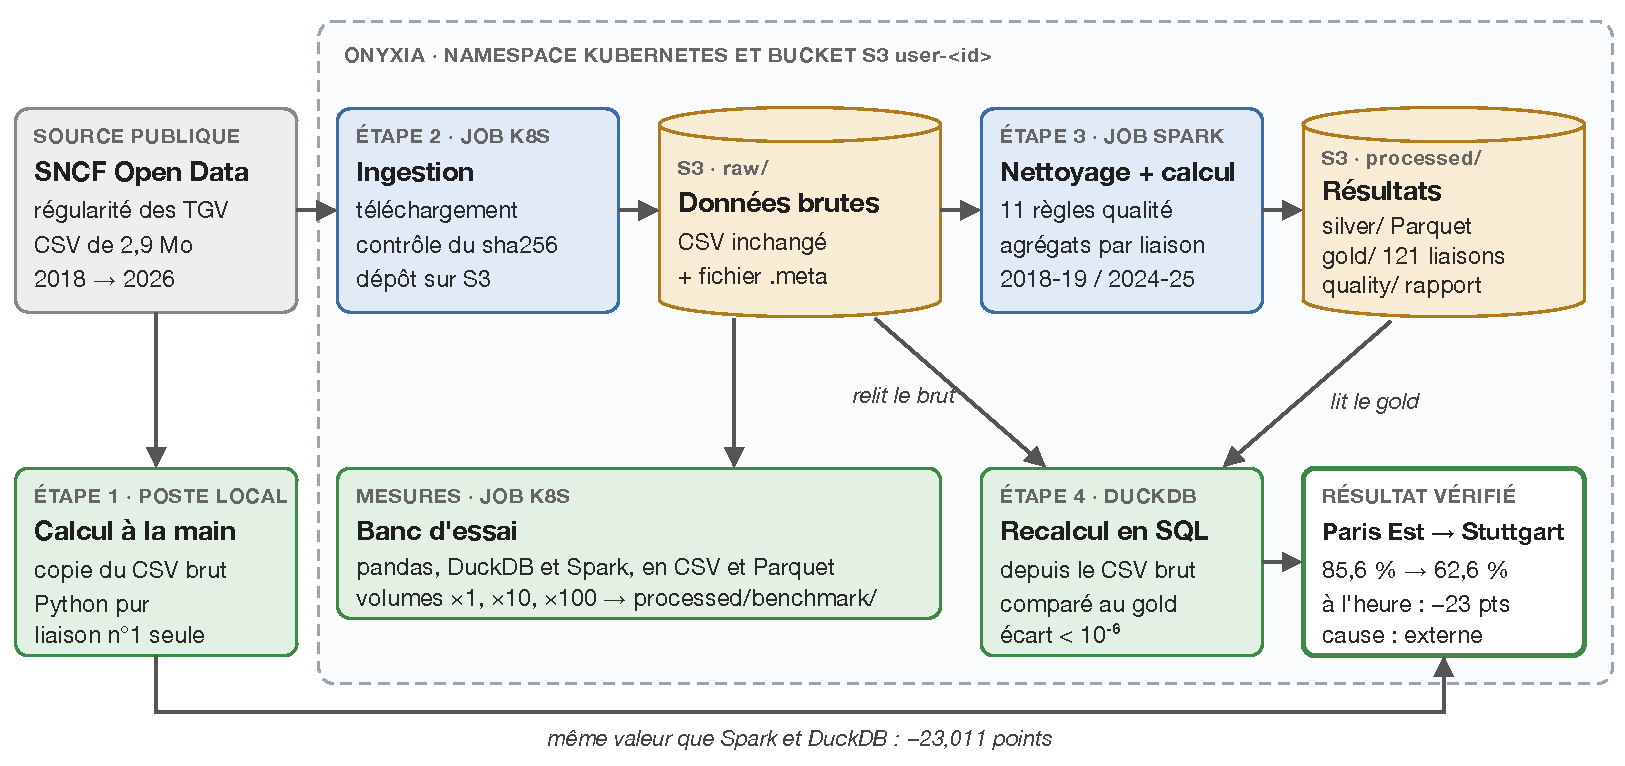
\includegraphics[width=\linewidth]{schema_pipeline.pdf}
\caption{Schéma du pipeline : la chaîne principale en haut, les contrôles en bas. Les étapes portent les mêmes numéros que dans \code{src/run\_pipeline.sh}.}
\label{fig:pipeline}
\end{figure}

Le pipeline suit l'\textbf{architecture médaillon} vue en cours : \code{raw/} joue le rôle de la couche \emph{bronze} (données brutes, inchangées), \emph{silver} contient les données nettoyées et typées, et \emph{gold} les agrégats qui répondent à la question. Tout tourne sur Onyxia, dans le namespace de l'utilisateur, et \code{bash src/run\_pipeline.sh} enchaîne les étapes 2 à 4 en 3 minutes environ.
\begin{itemize}
  \item \textbf{Étape 2, ingestion (Job Kubernetes).} Un initContainer \code{curl} télécharge le CSV à la source et refuse le fichier si son sha256 ou sa taille ne correspondent pas. Un conteneur \code{aws-cli} le dépose ensuite tel quel dans \code{raw/}, accompagné d'un fichier \code{.meta} (source, date, taille, sha256).
  \item \textbf{Étape 3, transformation (Job Kubernetes Spark).} Spark lit le brut avec un schéma explicite, applique les 11 règles de qualité (§\ref{sec:qualite}), écrit la couche silver en Parquet partitionné par année, puis la couche gold (121 liaisons classées) et le rapport qualité dans \code{quality/}.
  \item \textbf{Étape 4, vérification (DuckDB).} DuckDB relit le CSV brut, refait tout le calcul en SQL et le compare au gold, liaison par liaison (§\ref{sec:resultats}).
\end{itemize}

\textbf{Choix techniques et alternatives écartées.} Les alternatives sont mesurées, pas supposées : un Job Kubernetes dédié (\code{benchmark-tgv}, 2 CPU et 2 Go) refait le même calcul (ponctualité par liaison, top 1) avec pandas, DuckDB et Spark, sur le CSV et le Parquet, au volume réel puis à ×10 et ×100. Chaque mesure est la médiane de 3 passages, dans un processus neuf (preuve 06).

{\footnotesize
\begin{tabular*}{\linewidth}{@{\extracolsep{\fill}}l *{6}{r} r@{}}
\toprule
Temps médian (s) & \multicolumn{2}{c}{×1 (2,8 / 1,3 Mo)} & \multicolumn{2}{c}{×10 (28 / 3,9 Mo)} & \multicolumn{2}{c}{×100 (277 / 38 Mo)} & RAM max \\
\cmidrule(lr){2-3}\cmidrule(lr){4-5}\cmidrule(lr){6-7}
 & CSV & Parquet & CSV & Parquet & CSV & Parquet & ×100 Parquet \\
\midrule
pandas & 0,14 & 0,07 & 1,03 & 0,23 & 9,40 & 2,12 & 797 Mo \\
DuckDB & 0,18 & \textbf{0,06} & 0,43 & \textbf{0,08} & 2,33 & \textbf{0,21} & \textbf{78 Mo} \\
Spark \code{local[2]} & 3,50 & 3,26 & 4,29 & 3,92 & 11,08 & 6,89 & 1\,097 Mo \\
\bottomrule
\end{tabular*}}
{\footnotesize Spark ajoute environ 10,8 s de démarrage de la JVM, non compté ici. Les trois moteurs trouvent les mêmes 121 liaisons et le même n°1 (−23,011 points) à chaque échelle.\par}

{\footnotesize
\begin{tabularx}{\linewidth}{@{}>{\raggedright\arraybackslash}p{3.1cm} >{\raggedright\arraybackslash}p{3.6cm} >{\raggedright\arraybackslash}X@{}}
\toprule
\textbf{Choix retenu} & \textbf{Alternative écartée} & \textbf{Ce qui a tranché} \\
\midrule
Ingestion par un Job Kubernetes, depuis la source & \code{aws s3 cp} lancé à la main depuis le terminal & Le Job est déclaratif et rejouable, et il vérifie le sha256 \emph{avant} le dépôt, sans copie sur un poste (20 s, preuve 02). \\
Spark pour la transformation & pandas ; DuckDB & À notre volume, Spark est le plus lent (3,3 s + 10,8 s de JVM, contre 0,06 s pour DuckDB). Nous le gardons parce que c'est le seul des trois dont le même code passe sur plusieurs machines (§7). pandas est écarté car sa mémoire monte vite (797 Mo à ×100, contre 78 Mo pour DuckDB). \\
Spark \code{local[2]} dans un Job & executors Spark sur Kubernetes ; Spark dans le terminal VS Code & Les executors sont refusés : chacun demande 896 Mi de \code{requests.memory}, alors que le quota (200 Mi) est déjà pris par le service (preuve 07). Lancé dans le service, Spark a été tué faute de mémoire (OOMKilled : JVM de 2 Go + VS Code, au-delà de 2\,000 Mi). \\
Silver en Parquet & rester en CSV & Le fichier est 2,2 fois plus petit au volume réel et 7,3 fois à ×100. DuckDB le lit 11 fois plus vite à ×100 (0,21 s contre 2,33 s). \\
8 partitions + \code{repartition(annee)} & réglage par défaut (200 partitions) & 1\,799 fichiers Parquet de 13 Ko (23 Mo) et 174 s d'écriture sur S3, contre 9 fichiers (1,4 Mo) et 7,7 s : 23 fois plus rapide (preuve 06). \\
Spark + Jobs Kubernetes & dbt + DuckDB (TP5) & Très rapide à notre volume (DuckDB : 0,06 s) et tests de qualité intégrés, mais limité à une seule machine, comme DuckDB (§7). Pour un volume fixe et une équipe orientée SQL, dbt aurait aussi été un bon choix. \\
Vérification par DuckDB, depuis le brut & relancer Spark & Un autre moteur, un autre lecteur CSV et un autre code ne partagent pas les mêmes bugs. Si les deux concordent, c'est une vraie vérification. \\
Parquet partitionné & table Iceberg (TP8) & Une seule extraction figée, sans mise à jour ni besoin de revenir à une version antérieure : les snapshots d'Iceberg n'apportaient rien ici. Choix fait sur le besoin, sans mesure. \\
\bottomrule
\end{tabularx}}

% ---------------------------------------------------------------- 4
\section{Qualité des données}\label{sec:qualite}

Les 11 règles sont appliquées par Spark. Le nombre de lignes touchées est calculé à chaque exécution et écrit dans \code{processed/quality/} (preuve 04) ; nous l'avons recompté en Python, à l'identique. Aucune ligne n'est supprimée du silver : chaque défaut y est signalé par une colonne \code{q\_*}, ce qui permet de tout retracer.

{\footnotesize
\begin{tabularx}{\linewidth}{@{}l >{\raggedright\arraybackslash}X r >{\raggedright\arraybackslash}p{4.1cm}@{}}
\toprule
 & \textbf{Défaut, avec un exemple réel} & \textbf{Lignes} & \textbf{Traitement} \\
\midrule
R01 & BOM UTF-8 en tête du fichier : un lecteur qui ne le gère pas nomme la 1\textsuperscript{re} colonne «~\code{\textbackslash ufeffdate}~» au lieu de «~\code{date}~» & fichier & schéma explicite des 26 colonnes \\
R02 & commentaires sur plusieurs lignes : une lecture naïve trouve 15\,418 lignes au lieu de 12\,907 & 351 & lecture \code{multiLine=true} \\
R03 & aucun train prévu : 2020-04, \textsc{Francfort}\,$\rightarrow$\,\textsc{Paris Est}, 0 prévu mais 12 annulés & 73 & exclues des taux \\
R04-05 & annulations $>$ prévus, et retards $>$ trains circulés : les mêmes lignes (toutes en 2020, dont 50 en avril) & 63 & incluses dans R03 \\
R06 & plus de retards de plus de 15 min que de retards au total : 2018-01, \textsc{Grenoble}\,$\rightarrow$\,\textsc{Paris Lyon}, 25 contre 23 & 31 & plafonné au total \\
R07 & retards de plus de 30 / 60 min négatifs ou non emboîtés : 2025-01, \textsc{Lausanne}\,$\rightarrow$\,\textsc{Paris Lyon}, $-4$ trains à plus de 30 min ; 355 de ces lignes datent de janvier à mars 2025 & 357 & mis à NULL (inutilisés dans le calcul) \\
R08 & trains en retard mais aucune cause renseignée : 2018-05, \textsc{Barcelona}\,$\rightarrow$\,\textsc{Paris Lyon}, 12 retards, 0\,\% partout & 80 & cause «~non renseignée~» \\
R09 & somme des 6 causes différente de 100\,\% : 2026-06, \textsc{Paris Montparnasse}\,$\rightarrow$\,\textsc{Laval}, 84,62\,\% & 9 & renormalisée à 100\,\% \\
R10 & même liaison et même mois en National \emph{et} en International (juillet à septembre 2025), par exemple \textsc{Paris Lyon}\,$\rightarrow$\,\textsc{Mâcon Loché} avec 96 + 94 trains & 84 & additionnés, et non dédoublonnés : supprimer une ligne aurait fait perdre la moitié des trains \\
R11 & retard moyen négatif : 2019-11, \textsc{Montpellier}\,$\rightarrow$\,\textsc{Paris Lyon}, $-30{,}5$ min & 2 & mis à NULL \\
\bottomrule
\end{tabularx}}
Au total, 73 lignes (0,6\,\%) sont exclues du calcul des taux, toutes en 2020, donc hors des deux périodes comparées.

% ---------------------------------------------------------------- 5
\section{Résultats et vérification}\label{sec:resultats}

\begin{figure}[h]
\centering
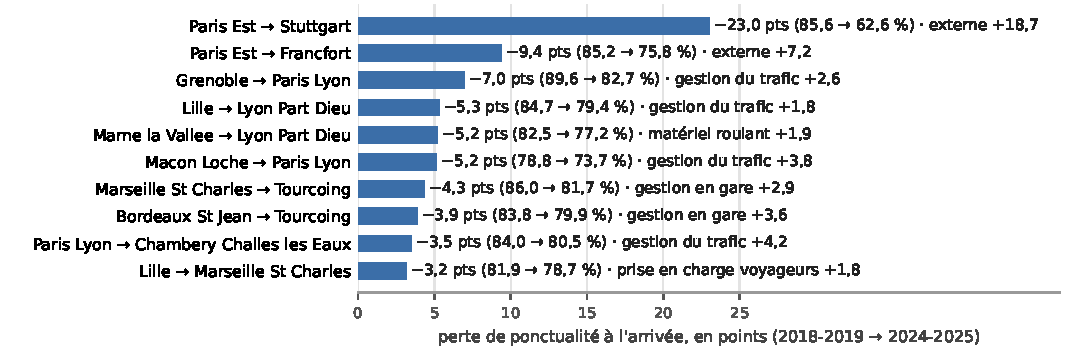
\includegraphics[width=\linewidth]{top10_degradation.pdf}
\caption{Les 10 liaisons qui ont le plus perdu : perte en points, ponctualité avant $\rightarrow$ après, et cause dont la contribution a le plus augmenté. Données : \code{gold/degradation\_liaisons} ; figure régénérée par \code{src/06\_figure\_top10.py}.}
\label{fig:top10}
\end{figure}

\textbf{Réponse à la question.} La dégradation est \emph{concentrée} sur quelques liaisons. Seules 38 liaisons sur 121 perdent en ponctualité, dont 18 de plus de 2 points. La variation médiane est de $+1{,}5$ point, et l'ensemble des liaisons comparées passe de 84,1\,\% à 85,6\,\%, un agrégat indicatif puisqu'un TGV peut compter dans plusieurs liaisons. \textbf{Les TGV vers l'Allemagne décrochent} : sur Paris Est $\rightarrow$ Stuttgart, la ponctualité passe de 85,6 à 62,6\,\% (les retards de plus de 15 min passent de 13,7 à 37,4\,\%), et 18,7 des 23,0 points perdus viennent des causes externes ; Francfort suit ($-9{,}4$ points, externe $+7{,}2$). Ces trains finissent leur trajet sur le réseau allemand, hors du périmètre de la SNCF, ce qui est cohérent avec une cause «~externe~», sans que les données permettent d'aller plus loin. \textbf{Ailleurs, ce sont les causes internes qui dominent} : sur les 38 liaisons dégradées, la cause principale est la gestion du trafic pour 15 d'entre elles, puis la gestion en gare (10). En moyenne pondérée par le trafic sur ces 38 liaisons, la gestion du trafic pèse $+0{,}95$ point, la prise en charge des voyageurs $+0{,}81$ et la gestion en gare $+0{,}61$, tandis que les causes externes reculent ($-0{,}54$). L'axe Paris-Lyon-Alpes revient souvent (Grenoble, Mâcon, Chambéry, Lyon).

\textbf{Vérification indépendante.} \textit{(1)} DuckDB relit le CSV brut, sans réutiliser le travail de Spark, refait le calcul en SQL et trouve les mêmes 121 liaisons, dans le même ordre, avec un écart maximal de 0 sur la ponctualité et de $1{,}4\cdot10^{-14}$ point sur les causes (arrondis machine). Le script échoue si un écart dépasse $10^{-6}$ (preuve 05). \textit{(2)} Un calcul à la main en Python pur, mois par mois, retrouve $-23{,}011$ points pour le n°1 et $-6{,}965$ pour le n°3 ; GitHub Actions le relance à chaque push (preuves 11-12). \textit{(3)} Dans le banc d'essai, pandas, DuckDB et Spark trouvent le même n°1 à toutes les échelles (preuve 06).

% ---------------------------------------------------------------- 6
\section{Limites}
\begin{itemize}
  \item \textbf{Données agrégées au mois.} Il n'y a aucune information par train, et la SNCF précise qu'on ne doit pas en déduire une régularité globale : nous ne comparons que des liaisons entre elles. Le seuil de retard dépend de la durée du trajet, mais la comparaison se fait liaison par liaison. Avec un seuil unique de 15 min (\code{delta\_retard15\_pts}, dans le gold), les deux premières liaisons sont les mêmes, et les six premières restent dans le top 9.
  \item \textbf{Causes.} Nous appliquons les pourcentages de causes au nombre de trains en retard, ce qui suppose une répartition proportionnelle. La catégorie «~externe~» est hétérogène, et le jeu de données ne permet pas d'en dire plus sur Stuttgart et Francfort.
  \item \textbf{Choix d'analyse.} Les bornes des périodes et le seuil de 18 mois sur 24 écartent 9 liaisons sur 130. Les corrections R06, R07 et R10 sont des interprétations, que nous documentons. Les petites liaisons, comme celles vers Tourcoing avec environ 550 trains par période, sont plus bruitées, et nous n'avons pas fait de test statistique de significativité.
\end{itemize}

% ---------------------------------------------------------------- 7
\section{Si les données étaient 100 fois plus volumineuses}

Avec 100 fois plus de données, on aurait environ 1,3 million de lignes, 277 Mo en CSV et 38 Mo en Parquet. Nous l'avons \emph{mesuré}, en répliquant le brut (tableau du §\ref{sec:pipeline}). \textbf{Une seule machine suffit encore} : DuckDB fait le calcul en 0,21 s avec 78 Mo de mémoire, et Spark en 6,9 s. pandas, en revanche, monte à 797 Mo, soit 40\,\% de la limite de 2 Go du pod. Ce qui changerait : \textbf{(1)} on convertirait en Parquet dès l'ingestion (7 fois plus petit) et on découperait \code{raw/} par mois, alimenté par un CronJob mensuel qui ne télécharge que le nouveau mois ; \textbf{(2)} il faudrait éviter \code{multiLine} sur un gros CSV, car Spark ne peut alors pas découper le fichier et le lit en une seule tâche ; \textbf{(3)} le réglage des partitions deviendrait indispensable, puisque le réglage par défaut produit déjà 1\,799 petits fichiers au volume réel ; \textbf{(4)} avec des ajouts chaque mois, un silver en Iceberg deviendrait utile (commits atomiques, snapshots, évolution du schéma) ; \textbf{(5)} DuckDB resterait adapté pour la vérification, mais le calcul à la main devrait lire le fichier en flux.
À ×100, DuckDB sur un seul nœud reste donc le choix le plus raisonnable. Spark distribué ne se justifierait que vers ×10\,000, soit environ 30 Go (une extrapolation que nous n'avons pas mesurée), quand une seule machine ne suffirait plus. Le même code tournerait alors avec des executors Kubernetes, à condition de relever le quota \code{requests.memory} du namespace, qui les bloque aujourd'hui (preuve 07). Les résultats, eux, ne changeraient pas : à chaque échelle, le n°1 reste le même.

% ---------------------------------------------------------------- annexe (dans les 4 pages)
\appendix
\section*{Annexe -- Preuves d'exécution et initiatives}\label{sec:preuves}

Les captures sont dans \code{evidence/} du dépôt, en taille réelle ; chaque numéro du tableau est un lien cliquable vers l'image. Les captures 01 à 10 viennent du terminal du service \code{vscode-pyspark}, dans le namespace \code{user-a-benatar-ece}, le 2026-11-17 entre 7\,h\,44 et 8\,h\,28. Le namespace et l'heure s'affichent dans l'invite et sur les deux premières lignes de chaque capture.

{\footnotesize
\begin{tabularx}{\linewidth}{@{}r >{\raggedright\arraybackslash}X >{\raggedright\arraybackslash}p{4.3cm}@{}}
\toprule
\textbf{N°} & \textbf{Ce que montre la capture} & \textbf{Composant / exigence} \\
\midrule
\href{https://raw.githubusercontent.com/LouisAmedeo/bigdata_project/main/evidence/01_clone_depot.png}{01} & \code{git clone} du dépôt public dans le service, puis l'historique & reproduction \\
\href{https://raw.githubusercontent.com/LouisAmedeo/bigdata_project/main/evidence/02_ingest_job_logs.png}{02} & Job \code{ingest-raw-tgv} \emph{Complete} : téléchargement, sha256, dépôt & Kubernetes (ingestion) \\
\href{https://raw.githubusercontent.com/LouisAmedeo/bigdata_project/main/evidence/03_s3_raw_listing.png}{03} & \code{aws s3 ls} de \code{raw/} : CSV et \code{.meta}, objet relu sur S3 & \textbf{bucket S3 : raw} \\
\href{https://raw.githubusercontent.com/LouisAmedeo/bigdata_project/main/evidence/04_spark_job_logs.png}{04} & Job \code{transform-spark-tgv} : rapport qualité R01-R11, top 10, sorties & Spark \\
\href{https://raw.githubusercontent.com/LouisAmedeo/bigdata_project/main/evidence/05_duckdb_verification.png}{05} & DuckDB depuis le brut : \code{VERIFICATION OK} sur 121 liaisons & DuckDB, vérification \\
\href{https://raw.githubusercontent.com/LouisAmedeo/bigdata_project/main/evidence/06_benchmark_job.png}{06} & Job \code{benchmark-tgv} : pandas / DuckDB / Spark, ×1 ×10 ×100, petits fichiers & mesures (§3, §7) \\
\href{https://raw.githubusercontent.com/LouisAmedeo/bigdata_project/main/evidence/07_spark_executors_quota.png}{07} & executors Spark sur Kubernetes refusés par le quota & alternative écartée \\
\href{https://raw.githubusercontent.com/LouisAmedeo/bigdata_project/main/evidence/08_relance_run_pipeline.png}{08} & \code{run\_pipeline.sh 3} : reprise à l'étape 3, tout se termine bien & relance idempotente \\
\href{https://raw.githubusercontent.com/LouisAmedeo/bigdata_project/main/evidence/09_kubectl_jobs_quota.png}{09} & \code{kubectl get jobs,pods}, ConfigMaps, Secret, quota du namespace & Kubernetes \\
\href{https://raw.githubusercontent.com/LouisAmedeo/bigdata_project/main/evidence/10_s3_processed_listing.png}{10} & \code{aws s3 ls --recursive} : \code{raw/} et \code{processed/} (silver, gold, quality\ldots) & \textbf{bucket S3 : processed} \\
\href{https://raw.githubusercontent.com/LouisAmedeo/bigdata_project/main/evidence/11_github_actions_run.png}{11}-\href{https://raw.githubusercontent.com/LouisAmedeo/bigdata_project/main/evidence/12_github_actions_verif_ok.png}{12} & GitHub Actions : même sha256, vérification à la main OK & reproduction hors Onyxia \\
\bottomrule
\end{tabularx}}

\textbf{Initiatives (au-delà du minimum demandé) :} extraction figée et sha256 contrôlé à chaque ingestion ; 11 règles qualité, chacune avec son nombre de lignes, et aucune ligne perdue ; banc d'essai à trois moteurs et trois échelles ; test des petits fichiers (de 1\,799 à 9) ; executors Kubernetes testés puis écartés, preuve du refus à l'appui ; pipeline relançable à n'importe quelle étape ; double vérification, par DuckDB et à la main ; figure du rapport régénérée par un script depuis le brut ; intégration continue GitHub Actions (\url{https://github.com/LouisAmedeo/bigdata_project/actions}).

\textbf{Organisation du binôme.} Le projet a été mené à deux, et la plupart des étapes ont été faites en séance commune : choix du sujet et des données, conception du pipeline, écriture et exécution des scripts sur Onyxia, vérifications et rédaction. Chacun a ensuite pris en main plus particulièrement certaines parties. Louis s'est occupé de la préparation et du figeage des données, des vérifications indépendantes (calcul à la main, GitHub Actions), du schéma et de la mise en forme du rapport. Arthur s'est occupé des Jobs Kubernetes, du traitement Spark, de la vérification DuckDB et du banc d'essai. Chaque partie a été relue et validée par l'autre, et l'historique Git montre les contributions des deux.



\end{document}
